\documentclass[10pt,a4paper]{report}
\usepackage[T1]{fontenc}
\usepackage{graphicx}
\usepackage{hyperref}
\usepackage{cleveref}
\usepackage{float}

\title{Report}
\author{Haoyu Huang}

\begin{document}
	\maketitle
	\newpage
	\tableofcontents
	\newpage
	
	\section{Step 1}
	
	\subsection{Drawing the Box Plots}
		
		\begin{figure}
			\centering
			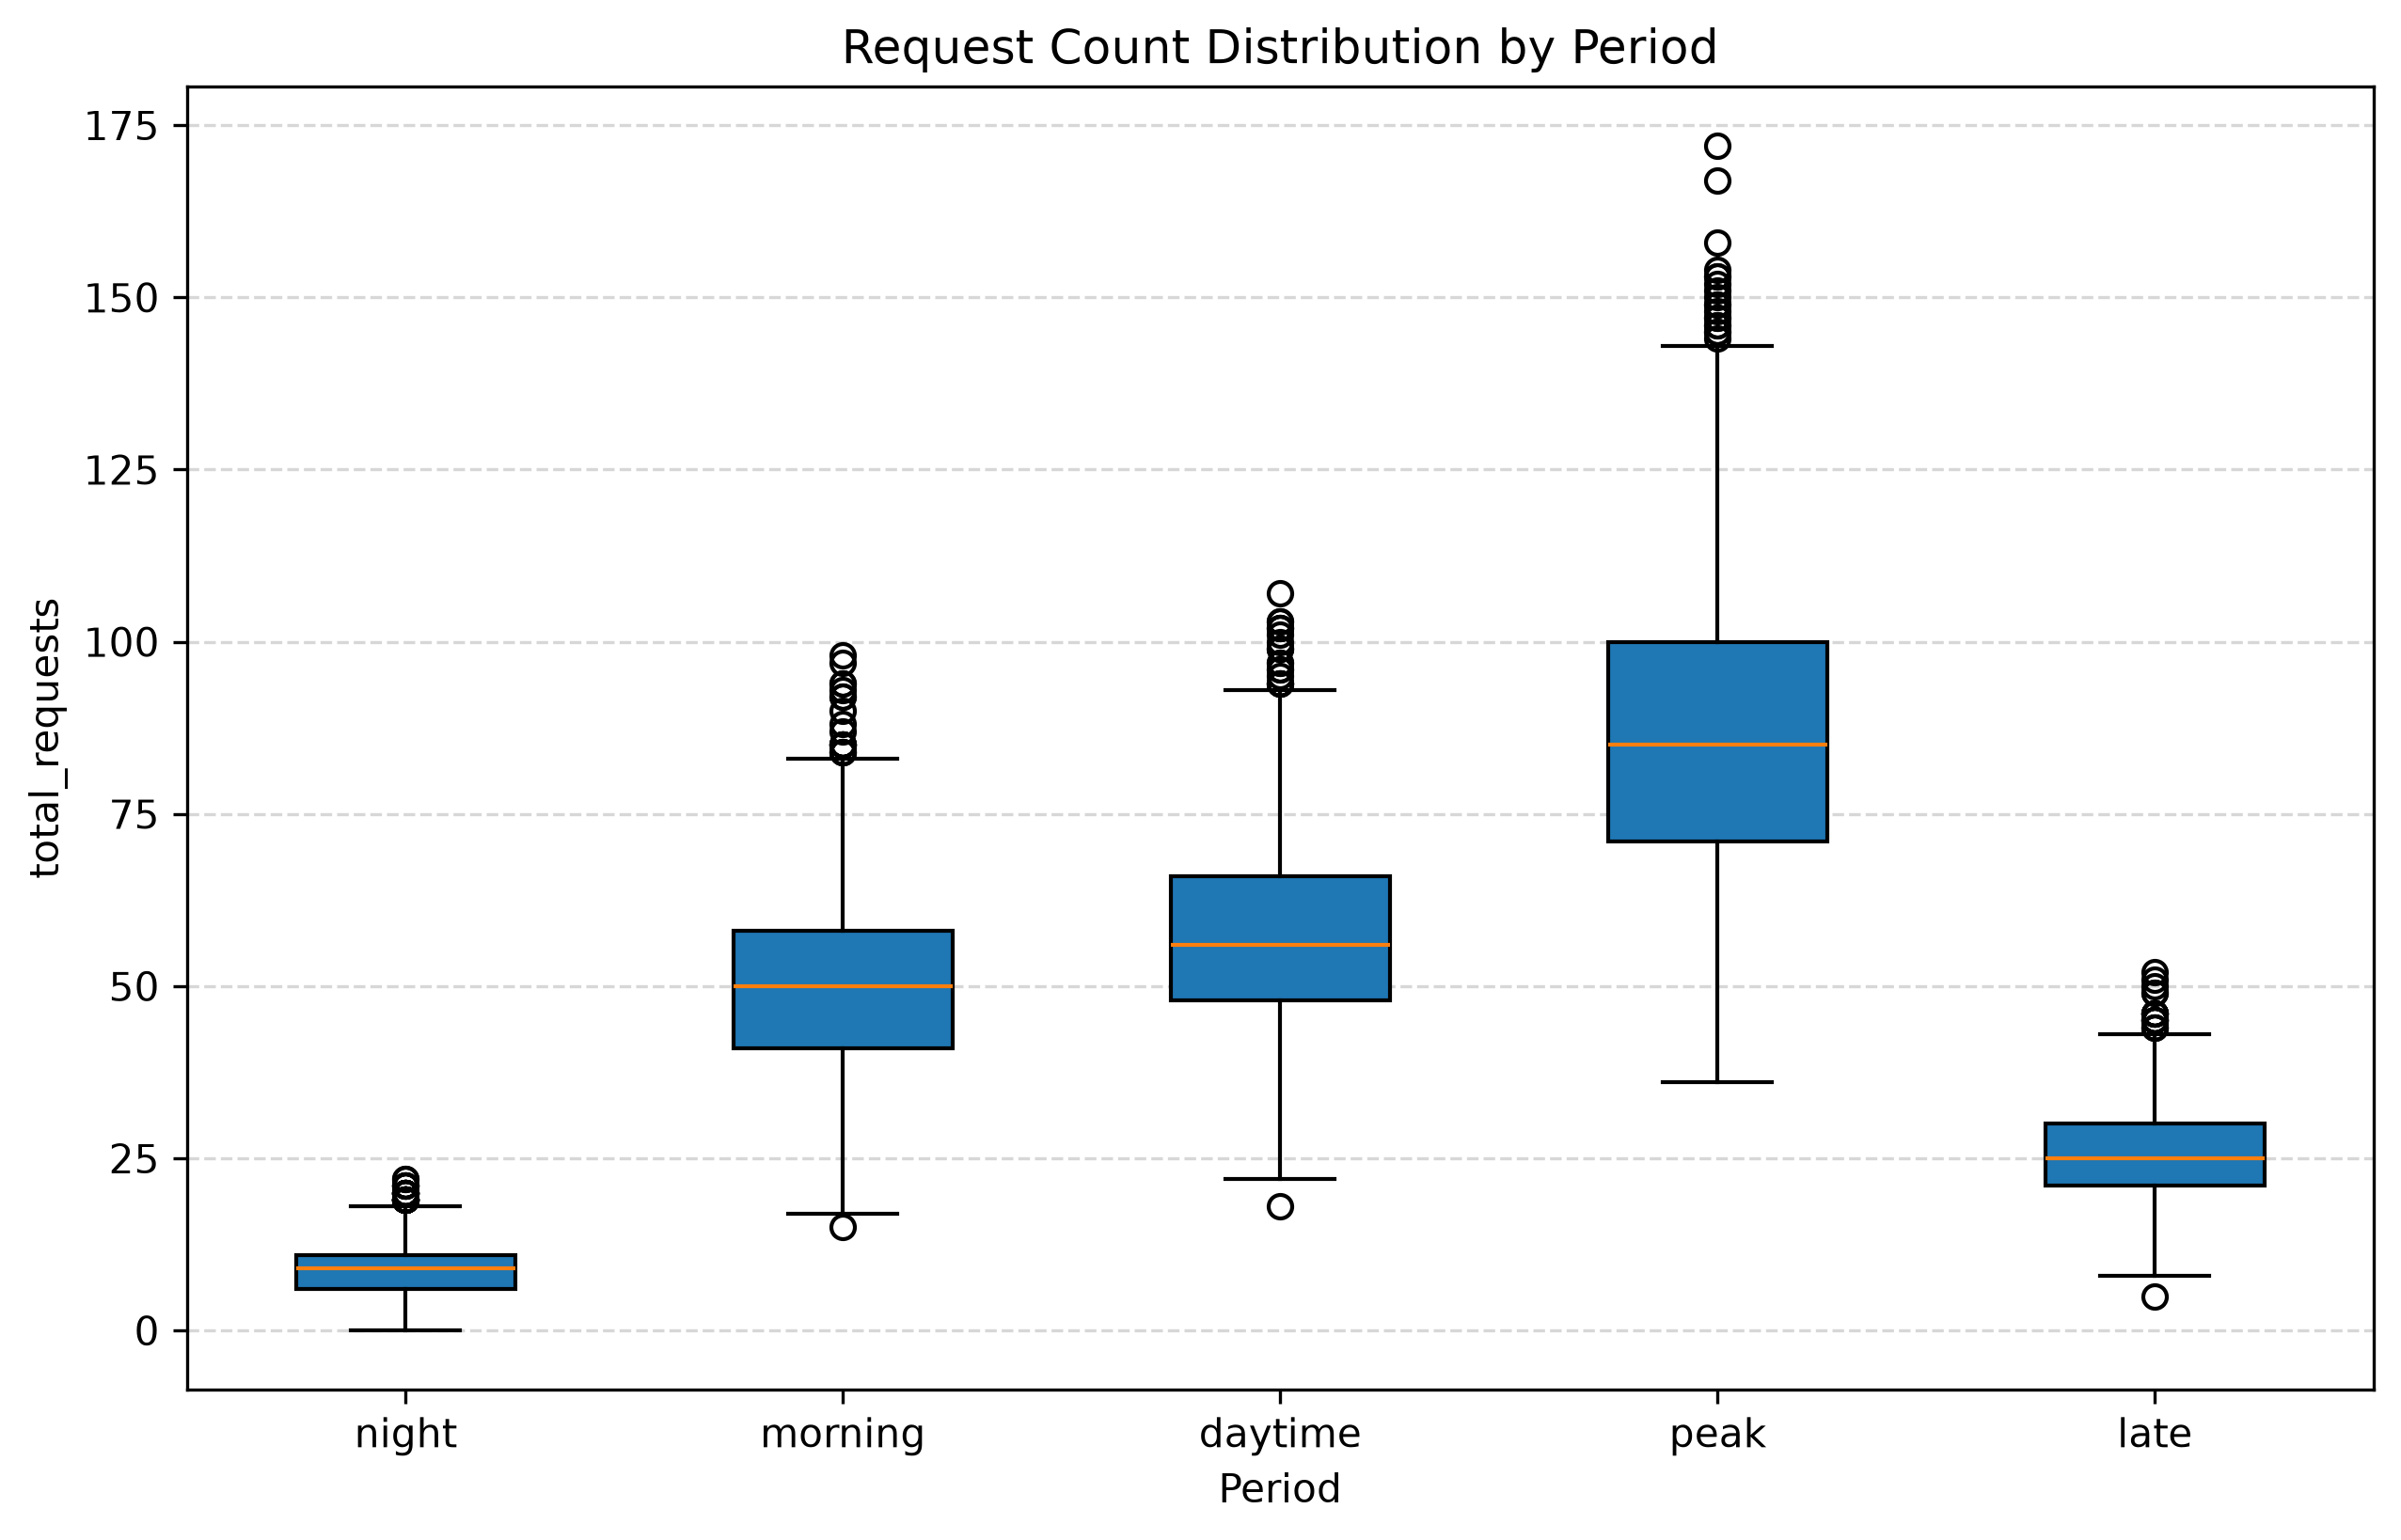
\includegraphics[width=0.7\linewidth]{../graphs/text_requests_boxplot}
			\caption{Box plots of text requests}
			\label{fig:textrequestsboxplot}
		\end{figure}
		
		\begin{figure}
			\centering
			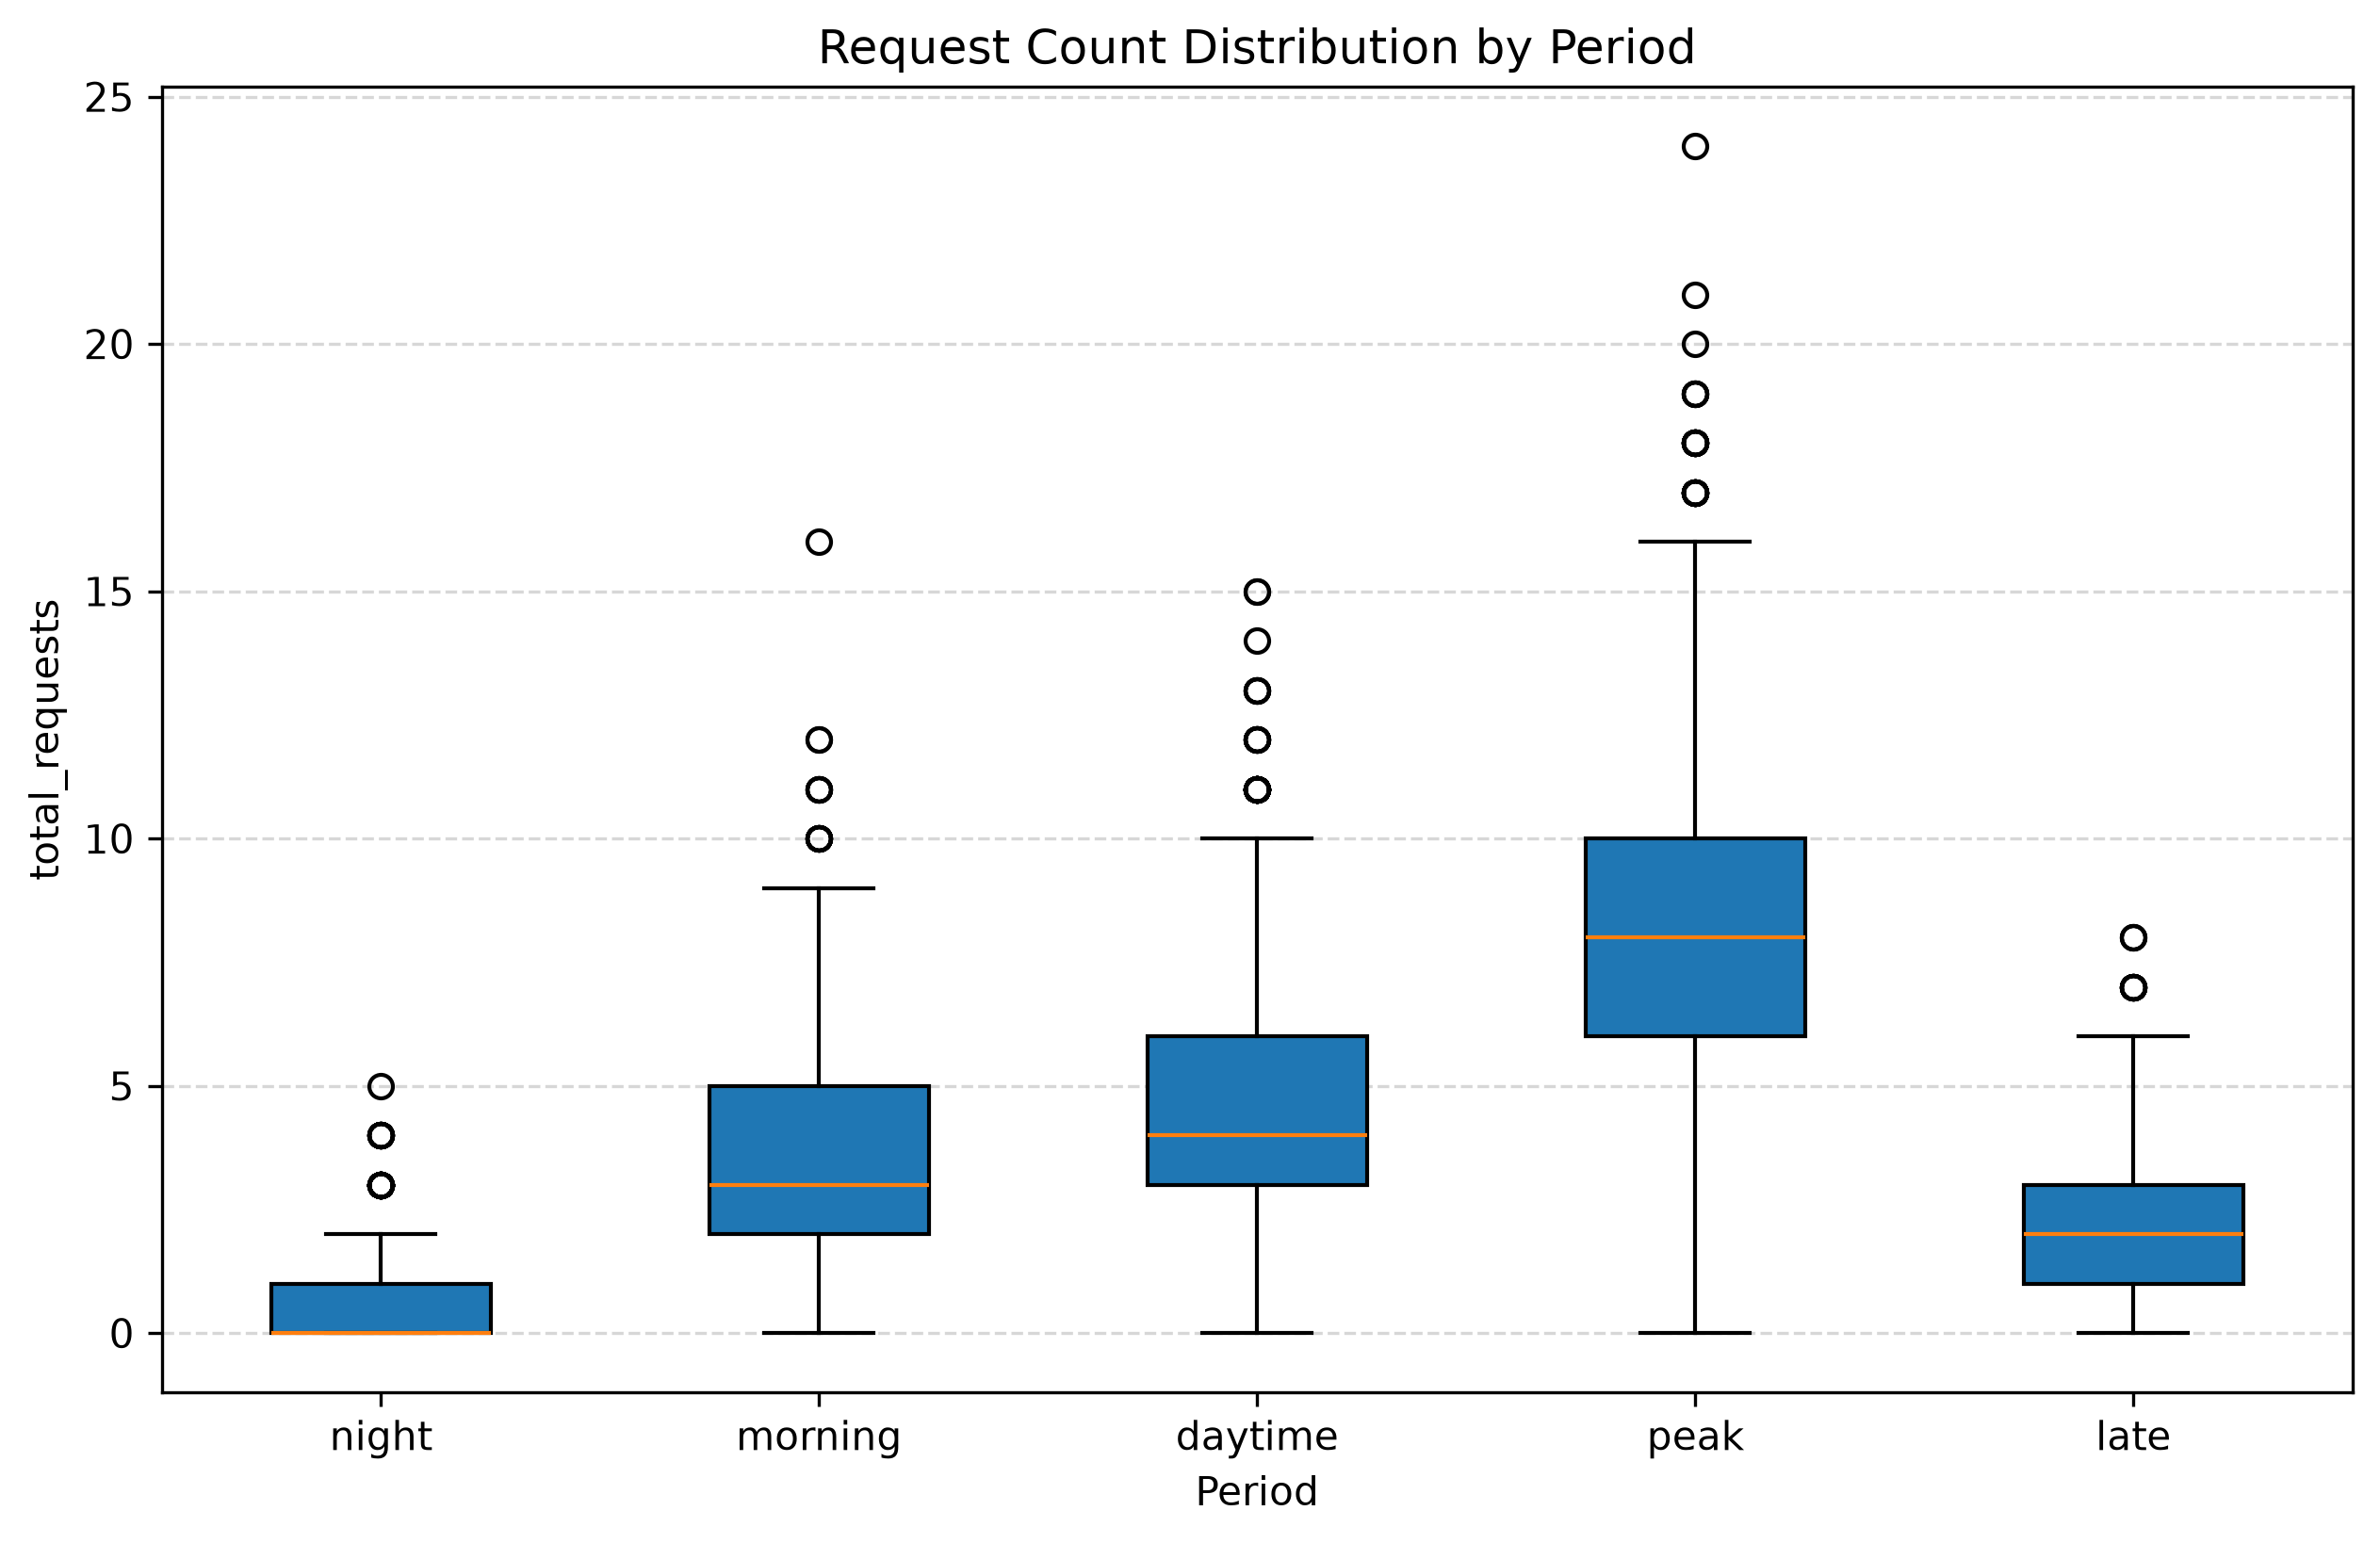
\includegraphics[width=0.7\linewidth]{../graphs/image_requests_boxplot}
			\caption{Box plots of image requests}
			\label{fig:imagerequestsboxplot}
		\end{figure}
		
		The box plots for the two types of requests are presented in
		\cref{fig:textrequestsboxplot} and \cref{fig:imagerequestsboxplot},
		respectively. It is evident that an analysis restricted to peak
		hours on weekdays alone cannot adequately illustrate the actual
		trends in request volumes.
	
	\subsection{Establish Poisson distribution}
		Poisson distributions are assumed for $N_t$ and $N_i$,
		specifically,
		
		\[
		P(N_t=k) = \frac{\lambda_t^k e^{-\lambda_t}}{k!},
		\]
		
		\[
		P(N_i=k) = \frac{\lambda_i^k e^{-\lambda_i}}{k!}.
		\]
		
		The parameters $\lambda_t$ and $\lambda_i$ can be estimated
		using the sample mean:
		
		\[
		\hat{\lambda} = \frac{1}{n}\sum_{i=1}^{n}N_i.
		\]
		
		The 95\% confidence interval for the Poisson parameter
		$\lambda$ can be approximated using the normal approximation:
		
		\[
		CI_{95\%} =
		\left[
		\hat{\lambda} - 1.96\sqrt{\frac{\hat{\lambda}}{n}},
		\hat{\lambda} + 1.96\sqrt{\frac{\hat{\lambda}}{n}}
		\right].
		\]
	
	\section{Step 2}
	\subsection{Report for service time}

		\begin{figure}[H]
			\centering
			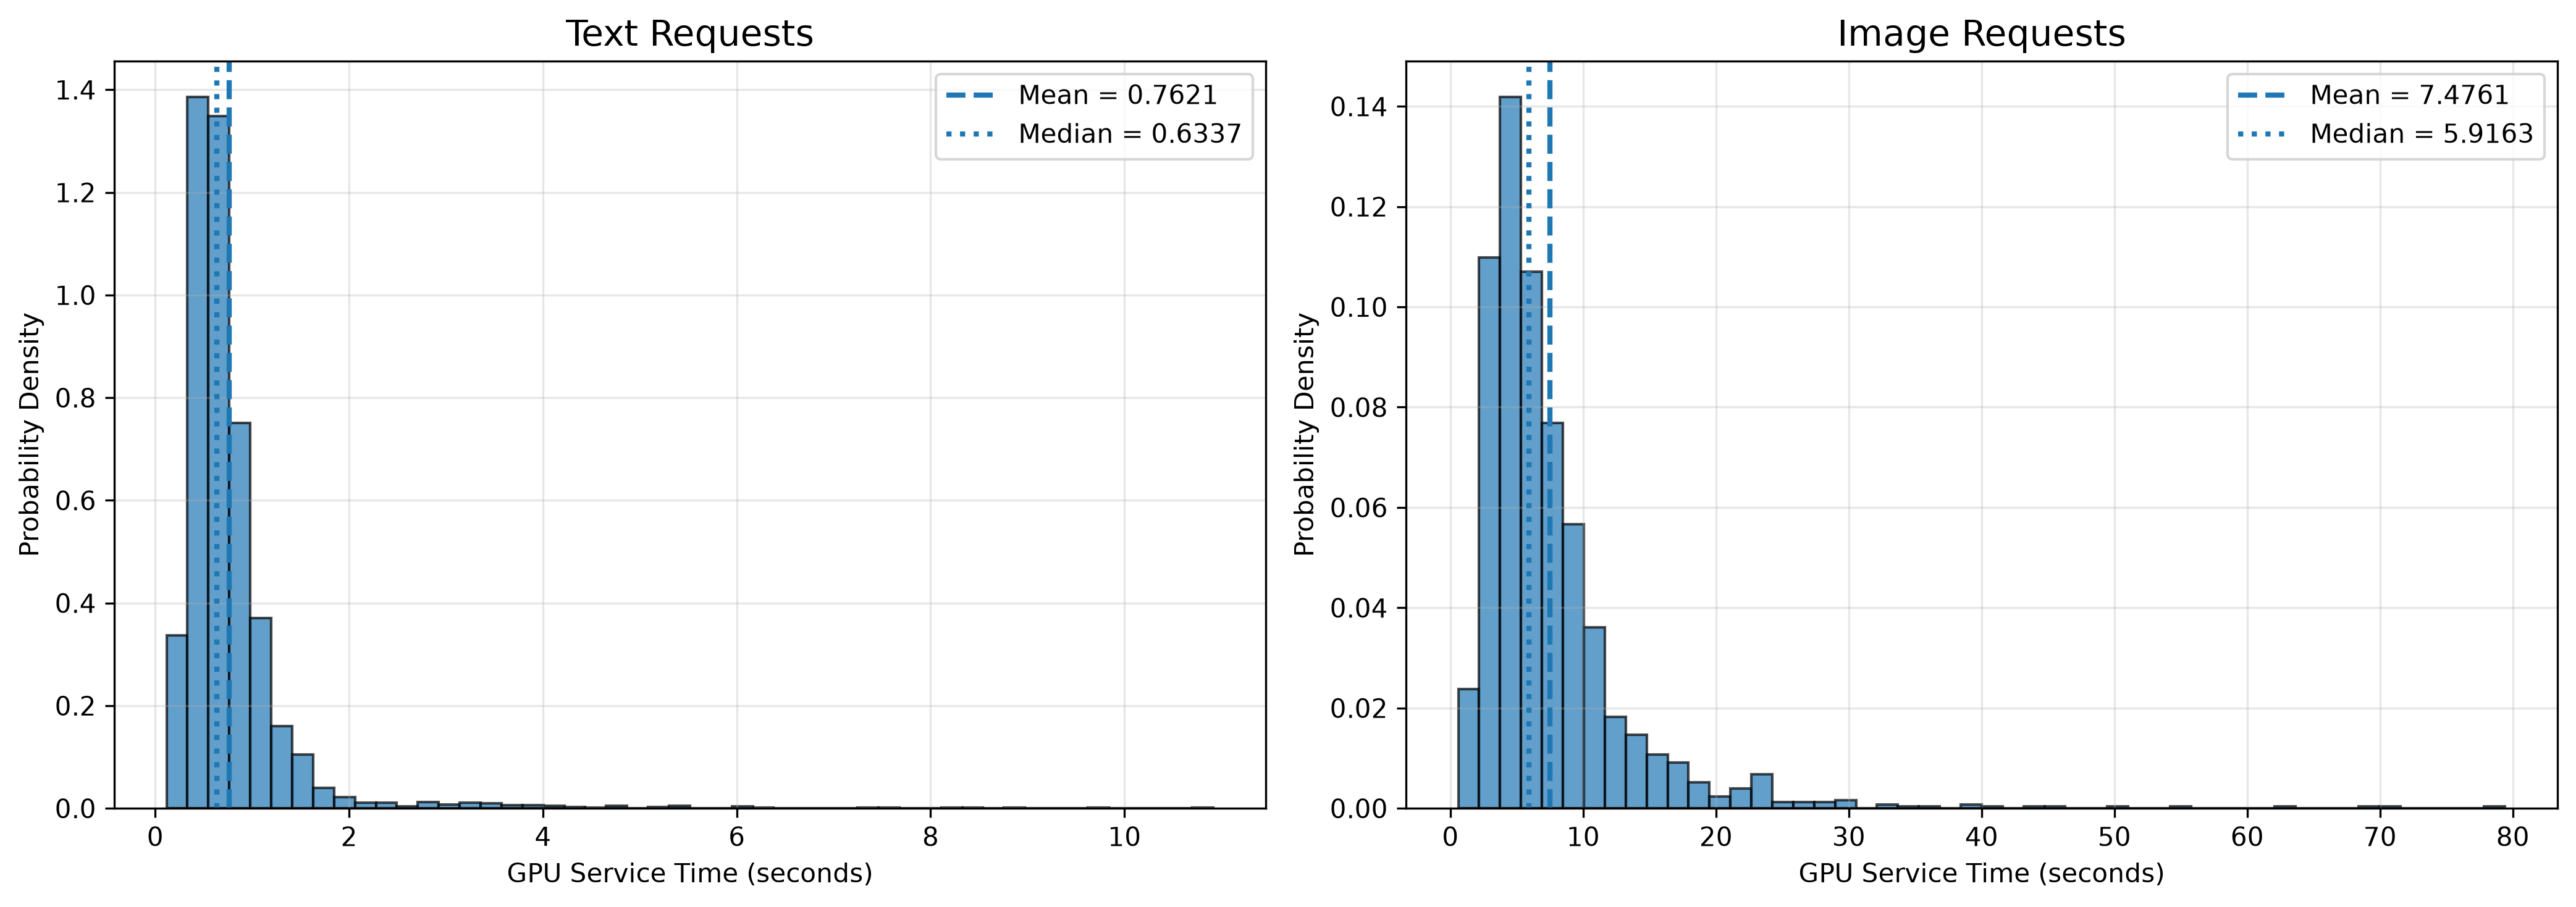
\includegraphics[width=1\linewidth]{../graphs/service_time_report}
			\caption{Histogram of two types of requests}
			\label{fig:servicetimereport}
		\end{figure}
		
			\begin{table}[htbp]
			\centering
			\caption{Descriptive Statistics of Text and Image Request Durations (seconds)}
			\label{tab:request_statistics}
			\begin{tabular}{ccccccc}
				\hline
				Type & Size & Mean (s) & Std (s)
				& Median (s) & 95\% (s) & 99\% (s) \\
				\hline
				Text  & 4000 & 0.762147 & 0.628502 & 0.633650 & 1.464310 & 3.528130 \\
				Image & 1600 & 7.476124 & 6.247750 & 5.916300 & 17.529665 & 29.749451 \\
				\hline
			\end{tabular}
		\end{table}
	
	\subsection{Report for cold start service time}
	\subsection{Establish Probability Model}
	\subsection{Estimate Model Parameters}
\end{document}